\documentclass[12pt, a4paper]{article}
\usepackage{ctex}
\usepackage{amsmath, amssymb}
\usepackage{geometry}
\geometry{left=2cm, right=2cm, top=2.5cm, bottom=2.5cm}
\usepackage{tikz}
\usepackage{multicol}

\title{\vspace{-2cm}第二讲 立体几何中的向量方法}
\author{}
\date{}

\begin{document}
\maketitle
\vspace{-1.5cm}

\noindent\textbf{方向向量与法向量\quad 空间中平行、垂直与空间向量的关系\quad 角度问题}

\vspace{0.3cm}
\hrule
\vspace{0.5cm}

\section*{1. 方向向量与法向量}

\begin{minipage}[t]{0.45\textwidth}
    \textbf{直线的方向向量}：$A, B$为直线上不同的两点，则$\overrightarrow{AB}$即方向向量之一。\\
    
    \textbf{平面的法向量}：$l \perp \text{平面}$，则与$l$平行的非零向量为平面的法向量。\\
    
    \textbf{法向量求法}：
    \begin{enumerate}
        \item 表示点坐标
        \item 表示两条边的方向向量
        \item 设 $\vec{n} = (x, y, z)$ 
        $$
        \begin{cases} 
        \vec{n} \cdot \text{方向向量}_1 = 0 \\ 
        \vec{n} \cdot \text{方向向量}_2 = 0 
        \end{cases}
        $$
        \item 赋值求解
    \end{enumerate}
    \vspace{0.2cm}
    
    \textbf{建系语言}：以 $\dots$ 为原点，$\overrightarrow{\dots}, \overrightarrow{\dots}, \overrightarrow{\dots}$ 方向分别为主轴 $x, y, z$ 轴的正方向建立如图空间直角坐标系。
\end{minipage}%
\hfill
\begin{minipage}[t]{0.5\textwidth}
    \textbf{例题}：正方体，两个三等分点，平面$AEF$的法向量？

    \textbf{解}：设边长为 3，$A(3, 0, 0)$，$E(3, 3, 1)$，$F(0, 3, 2)$
    
    $$ \overrightarrow{AE} = (0, 3, 1), \quad \overrightarrow{FE} = (3, 0, -1) $$
    
    设平面 $AEF$ 的一个法向量为 $\vec{n} = (x, y, z)$，则
    $$
    \begin{cases}
    \vec{n} \cdot \overrightarrow{AE} = 0 \\
    \vec{n} \cdot \overrightarrow{FE} = 0
    \end{cases}
    \Rightarrow
    \begin{cases}
    3y + z = 0 \\
    3x - z = 0
    \end{cases}
    $$
    
    令 $z = 3$，得 $x = 1, y = -1$。\\
    $\therefore \vec{n} = (1, -1, 3)$

    \vspace{0.5cm}
    \begin{center}
    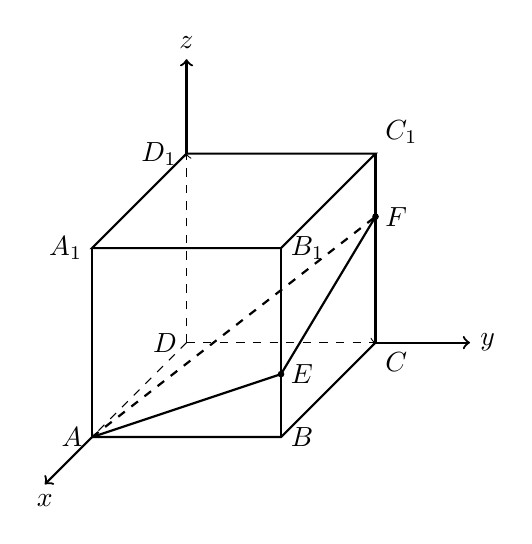
\begin{tikzpicture}[scale=0.8, x={(-0.5cm,-0.5cm)}, y={(1cm,0cm)}, z={(0cm,1cm)}]
        % 坐标点定义
        \coordinate (D) at (0,0,0);
        \coordinate (A) at (3,0,0);
        \coordinate (B) at (3,3,0);
        \coordinate (C) at (0,3,0);
        \coordinate (D1) at (0,0,3);
        \coordinate (A1) at (3,0,3);
        \coordinate (B1) at (3,3,3);
        \coordinate (C1) at (0,3,3);
        
        % 三等分点 E 和 F
        \coordinate (E) at (3,3,1); % E 在 BB1 上
        \coordinate (F) at (0,3,2); % F 在 CC1 上
        
        % 坐标轴 (内部虚线，外部实线)
        \draw[->, dashed] (D) -- (A);
        \draw[->, thick] (A) -- (4.5,0,0) node[below] {$x$};
        \draw[->, dashed] (D) -- (C);
        \draw[->, thick] (C) -- (0,4.5,0) node[right] {$y$};
        \draw[->, dashed] (D) -- (D1);
        \draw[->, thick] (D1) -- (0,0,4.5) node[above] {$z$};
        
        % 正方体可见边
        \draw[thick] (A) -- (B) -- (C);
        \draw[thick] (A) -- (A1);
        \draw[thick] (B) -- (B1);
        \draw[thick] (C) -- (C1);
        \draw[thick] (A1) -- (B1) -- (C1) -- (D1) -- cycle;
        
        % 顶点标签
        \node[left] at (A) {$A$};
        \node[right] at (B) {$B$};
        \node[below right] at (C) {$C$};
        \node[left] at (D) {$D$};
        \node[left] at (A1) {$A_1$};
        \node[right] at (B1) {$B_1$};
        \node[above right] at (C1) {$C_1$};
        \node[left] at (D1) {$D_1$};
        
        % 平面 AEF (可见边界为实线，不可见为虚线)
        \draw[thick, dashed] (A) -- (F); % 穿过体内部
        \draw[thick] (A) -- (E);         % 前面
        \draw[thick] (E) -- (F);         % 右侧面
        
        % 标注 E, F 点
        \node[right] at (E) {$E$};
        \node[right] at (F) {$F$};
        \fill (E) circle (1.5pt);
        \fill (F) circle (1.5pt);
    \end{tikzpicture}
    \end{center}
\end{minipage}

\end{document}
